\section{Integer Programs}
\label{sec:integer}

This chapter describes integer programs representing the problems discussed in previous chapters. In the next section we have a look at the implementation and practical results of some of the algorithms described throughout this thesis.\medskip

Let $G=(V,E,\gamma)$ an undirected graph with nonnegative node weights $c\colon V \to \RR_{\geq 0}$ and nonnegative edge weights $d\colon E \to \RR_{\geq 0}$. In all following IP/LP approaches, there are binary variables $y_v$ indicating whether a vertex $v$ is selected for the subgraph and binary variables $z_{e}$ indicating selected edges. By $y(S)$ we denote the sum of all variable values $y_v$ for $v \in S$: $y(S) \defeq \sum_{v \in S} y_v$. We formulate our IP/LP approaches as maximization problems, but they can be easily modified for solving minimization problems.

\subsection{Rooted Weighted Subgraph Problem}
\label{sec:integer:rooted}

Before we formulate an optimization problem for the \WSP\ or the \WISP, we start by looking at the rooted variants, namely the \RWSP\ and \RWISP. As it turns out those programs are slightly easier to set up since formulating connectivity constraints in the rooted case is more intuitive.\medskip

Formulating the objective function is straightforward

\begin{equation}
	\label{equation:objfunction}
	\begin{aligned}
		\sum_{e \in E} z_e \cdot c(e) + \sum_{v \in V} y_v \cdot d(v).
	\end{aligned}
\end{equation}

For the induced variant, \textsc{rwisp}, the requirement of the subgraph being induced can be modeled by the constraints

\begin{equation}
	\label{equation:induceconstraint}
	\begin{aligned}
		z_e &\geq y_u + y_v - 1 &&\text{ for all } e \in E \text{ with } \delta(e) = (u, v),\\
		z_e &\leq y_v &&\text{ for all } e \in E \text{ and } v \in \delta(e).
	\end{aligned}
\end{equation}

Given a root vertex $r \in V$, setting $y_r \defeq 1$ forces the $r$ to be in the solution. Thus, we are able ensure connectivity of the subgraph by the constraints

\begin{equation}
	\label{equation:connectivityconstraint}
	\begin{aligned}
		|V|\cdot z(\delta(S)) &\geq y(\bar{S}) &&\text{ for all } S \subseteq V \text{ with } r \in S.
	\end{aligned}
\end{equation}

Basically, one inequality is added for every cut $(S, \bar{S})$ of $V$ with $r \in S$. If there is a node $v \in \bar{S}$ with $y_v = 1$, this ensures that at least one of the edges in the cut has to be selected, too. Thus, the IP for \maxRWSP\ can be formulated as follows:

\begin{maxi}
	{}{\sum_{e\in E} z_e \cdot c(e) + \sum_{v\in V} y_v \cdot d(v)}{\label{opt:wsp}\tag{$\mathrm{CUT}_r$}}{}
	\addConstraint{z_e}{\geq y_u + y_v - 1}{\text{ for all } e \in E \text{ with } \delta(e) = (u, v)}
	\addConstraint{z_e}{\leq y_v}{\text{ for all } e \in E \text{ and } v \in \delta(e)}
	\addConstraint{y_r}{= 1}{}
	\addConstraint{|V|\cdot z(\delta(S))}{\geq y(\bar{S})}{\text{ for all } S \subseteq V \text{ with } r \in S}
	\addConstraint{z_e}{\in \BB}{\text{ for all } e \in E}
	\addConstraint{y_v}{\in \BB}{\text{ for all } v \in V.}
\end{maxi}

The IP \eqref{opt:wsp} can be easily modified for solving the minimization problems \minRWISP\ or the \minRWSP\ in the most direct way by minimizing the objective function \eqref{equation:objfunction}.

\begin{theorem}
	\label{thm:optwsp}
	 Given a root vertex $r \in V$, IP \eqref{opt:wsp} returns an optimal solution for the \RWISP. If the constraints \eqref{equation:induceconstraint} are dropped an optimal solution for \RWSP\ is returned.
\end{theorem}
\begin{proof}
	Let \ugraph\ be a graph and suppose we are given a feasible solution $(\bar{y}, \bar{z})$ for the IP \eqref{opt:wsp} representing a graph $H$. Then $\bar{y}_r = 1$ so the solution contains the root node $r \in H$. Further, suppose we have $\bar{z}_e = 0$ but $\bar{y}_u = \bar{y}_v = 1$ for two incident nodes $u, v \in \delta(e)$. But this is not possible due to the constraints \eqref{equation:induceconstraint} forcing $\bar{z}_e$ to be one. Conversely, the constraints \eqref{equation:induceconstraint} ensure that, if $\bar{z}_e = 1$, then $\bar{y}_u = 1$ and $\bar{y}_v = 1$ for $u, v \in \delta(e)$. So $H$ represents an induced subgraph of $G$. Now assume $H$ is not connected. Let $C$ be the connected component of $H$ containing $r$. Since $H$ is not connected $\bar{z}(\delta(S)) = 0$ and there are nodes $v \in \bar{C}$ with $\bar{y}_v = 1$, so $\bar{y}(\bar{C}) > 0$. This contradicts constraint \eqref{equation:connectivityconstraint}, and thus $H$ can only have one connected component.\medskip
	
	For the converse, assume we are given a connected induced subgraph of $H$ containing $r$. To obtain a feasible solution of we set $\bar{y}_v \eqdef 1$ for all $v \in H$ and $\bar{y}_v \eqdef 0$ for all $v \in G \setminus H$. Analogously, $\bar{z}_e \eqdef 1$ for all $e \in E(H)$ and $\bar{z}_e \eqdef 0$ for all $e \in E(G) \setminus E(H)$. Since $H$ is an induced subgraph, the constraints \eqref{equation:induceconstraint} are satisfied. Let $S$ be an arbitrary subset of $V$ with $r \in S$. If $y(\bar{S}) > 0$ at least one node of $H$ is in $\bar{S}$. But since $H$ is connected $\bar{z}(\delta(S)) > 0$ and therefore the constraint \eqref{equation:connectivityconstraint} is satisfied.\medskip
	
	If the constraints \eqref{equation:induceconstraint} are dropped, the subgraph is (not necessarily) induced, but all other arguments continue to hold.
\end{proof}

\begin{corollary}
	\label{corollary:optrwsp}
	In order to obtain a solution for the \WSP\ and the \WISP\ one can solve the IP \eqref{opt:wsp} obtaining solutions for the \RWSP\ and the \RWISP\ for all $r \in V$  and take the maximum or minimum of all those solutions.
\end{corollary}

In the above form it is not clear, that the relaxation of IP \eqref{opt:wsp} can be solved in polynomial time since it has an exponential number of constraints. The problem hereby are the connectivity constraints \eqref{equation:connectivityconstraint}, because they imply exponentially many inequalities. Our goal in the following is to separate the connectivity constraints and solve the remaining LP relaxation. We know that solving the separation problem in polynomial time is equivalent to solving the LP relaxation of the IP in polynomial time \cite{Wol97}.\medskip

Suppose we are given a $(\bar{y}, \bar{z})$ satisfying all constraints except the connectivity constraints \eqref{equation:connectivityconstraint}. We show that we can check in polynomial time whether $(\bar{y}, \bar{z})$ satisfy the connectivity constraints. To achieve this we introduce a flow to our graph. For this we need to modify our graph to be directed. The auxiliary graph $\overrightarrow{G} = (V, R)$ is defined as follows: Each edge $e = (u, v) \in E$ corresponds to two arcs $(u, v)$ and $(v, u)$ with lower capacity $\ell(uv) = \ell(vu) = 0$ and upper capacity $u(uv) = u(vu) = |V| \cdot \bar{z}(e)$. For all nodes $v \in V$ we add an arc $(v, r)$ incident to the root $r$. The lower capacity for those is $\ell(vr) = \bar{y}_v$ and the upper capacity is $u(vr) = \infty$ (see Figure \ref{fig:wspauxiliary}).

\begin{align*}
	\overrightarrow{G} &= (V, R) \text{ with }\\
	R &= \{ (u, v) | (u, v) \in E \} \cup \{ (v, u) | (u, v) \in E \} \cup \{ (v, r) | v \in V \},\\
	\ell(e) &= \begin{cases} 0, \text{ if } e = (u,v) \in E \text{ or } e = (u,v) \in E,\\
	\bar{y}_v, \text{ if } e = (v,r) \notin E\end{cases},\\
	u(e) &= \begin{cases} |V| \cdot \bar{z}(e), \text{ if } e = (u,v) \in E \text{ or } e = (u,v) \in E,\\
	\infty, \text{ if } e = (v,r) \notin E\end{cases}.
\end{align*}

\begin{figure}[H]
	\centering
	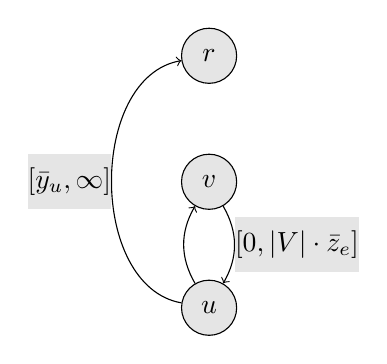
\begin{tikzpicture}[scale=1.6]
	\node[circle, draw] (r) at (0,2) {$r$};
	\node[circle, draw] (v) at (0,1) {$v$};
	\node[circle, draw] (u) at (0,0) {$u$};
	
	\path[->] (v) edge [bend left] node [right] {$[0, |V| \cdot \bar{z}_e]$} (u);
	\path[->] (u) edge [bend left] (v);
	\path[->] (u) edge [bend left=80] node [left] {$[\bar{y}_u, \infty]$} (r);
	\end{tikzpicture}	
	\caption{Construction of the auxiliary graph $G'$.}
	\label{fig:wspauxiliary}
\end{figure}

In order to prove the next lemma we need \textit{Hoffman’s circulation theorem}.

\begin{theorem}[Hoffman’s circulation theorem]
	\label{thm:hoffmancirculation}
	Let \graph\ be a directed graph and let $\ell, u \colon R \to \RR^+$ satisfy $\ell(r) < u(r)$ for every $r \in R$. Then either there exists a circulation $f \colon R \to \RR$ with $\ell(r) \leq f(r) \leq u(r)$ for every $r \in R$ or there exists $S \subseteq V$ such that
	$$u(S) \defeq \sum_{a \in \delta^+(S)} u(a) < \sum_{a \in \delta^-(S)} \ell(a) \eqdef \ell(\bar{S})$$
\end{theorem}

For the proof of Theorem \ref{thm:hoffmancirculation} we refer to \cite{AMO93}.

\begin{lemma}
	\label{lemma:circulation}
	Given $(\bar{y}, \bar{z})$ satisfying all constraints except the connectivity constraints \eqref{equation:connectivityconstraint} of the IP \eqref{opt:wsp}. There exists a circulation with respect to $\ell$ and $u$ in the auxiliary graph $\overrightarrow{G}$ if and only if $(\bar{y}, \bar{z})$ satisfies the connectivity constraint \eqref{equation:connectivityconstraint}.
\end{lemma}

\begin{proof}
	Assume $(\bar{y}, \bar{z})$ satisfies all constraints except the connectivity constraint of the IP \eqref{opt:wsp} and there exists a circulation with respect to $\ell$ and $u$ in $\overrightarrow{G}$. Using Hoffman’s circulation theorem \ref{thm:hoffmancirculation} it follows that $u(S) \geq \ell(\bar{S})$ for all $S \subseteq V$. Let $S \subseteq V$ be an arbitrary subset of $V$. If $r \in S$ we get that:
	$$\bar{y}(\bar{S}) = \sum_{v \in \bar{S}} \bar{y}_v = \ell(\bar{S}) \leq u(S) = \sum_{a \in \delta^+(S)} u(a) = |V| \cdot \bar{z}(\delta(S)).$$
	If $r \notin S$ there is nothing to show. Thus $(\bar{y}, \bar{z})$ is a feasible solution for the IP \eqref{opt:wsp}.\medskip
	
	Conversely, suppose that the connectivity constraint \eqref{equation:connectivityconstraint} holds for $(\bar{y}, \bar{z})$. Again, let $S \subseteq V$ be an arbitrary subset and assume $r \in S$. We have:
	\begin{align*}
		\ell(\bar{S}) &= \bar{y}(\bar{S})\\
		&\leq |V| \cdot \bar{z}(\delta(S))\\
		&= u(S)
	\end{align*}	
	If $r \notin S$, then $\ell(\bar{S}) = 0$ and $u(S) = |V| \cdot \bar{z}(\delta(S)) + \infty$, so $\ell(\bar{S}) \leq u(S)$ for all $S \subseteq V$. We obtain a feasible circulation with respect to $\ell$ and $u$ by applying Theorem \ref{thm:hoffmancirculation}.
\end{proof}

In order to show that the LP relaxation of IP \eqref{opt:wsp} is solvable in polynomial time, once again, we need to modify our graph $\overrightarrow{G}$ by adding a supersource $s$ and a supersink $t$. We obtain a new graph $G' = (V', R')$ where

\begin{align*}
	V' &\defeq V(\overrightarrow{G}) \cup \{s, t\}\\
	R' &\defeq R(\overrightarrow{G}) \cup \{(s, v),(v, t) \text{ for all } v \in V\}
\end{align*}

without lower capacities (i.e. $\ell'(r) = 0$ for all $r \in R'$) and

\begin{align*}
	u'(r) &= u(r) - \ell(r) && \text{ for all } r \in R(\overrightarrow{G}),\\
	u'(s,v) &= \ell(\delta^+(v)) = \sum_{r \in \delta^+(v)} \ell(r) && \text{ for all } v \in V(\overrightarrow{G}),\\
	u'(v,t) &= \ell(\delta^-(v)) && \text{ for all } v \in V(\overrightarrow{G}).\\
\end{align*}

\begin{lemma}
	\label{lemma:circulationflow}
	A circulation with respect to $\ell$ and $u$ in $\overrightarrow{G}$ exists if and only if the maximum $(s, t)$-flow in $G'$ (with respect to $u'$) has value $F \defeq \sum_{r \in R} \ell(r)$.
\end{lemma}
\begin{proof}
	Observe that $F = \sum_{r \in R} \ell(r) = \sum_{v \in V} \sum_{r \in \delta^+(v)} \ell(r) = \sum_{v \in V} \ell(\delta^+(v))$ and also $F = \sum_{v \in V} \ell(\delta^-(v))$, which means the arcs from $s$ and to $t$ are necessarily saturated in a flow of value $F$. Given a feasible circulation $\beta$ in $\overrightarrow{G}$, consider flow $f'$ in $G'$ with
	\begin{align*}
		f'(s,v) &= \ell(\delta^+(v)) && \text{ for all } v \in V,\\
		f'(v,t) &= \ell(\delta^-(v)) && \text{ for all } v \in V,\\
		f'(r) &= \beta(r) - \ell(r) && \text{ for all } r \in R.
	\end{align*}
	It follows that:
	\begin{align*}
		0 = f'(s,v) &= \ell(\delta^+(v)) = u'(s,v),\\
		0 = f'(v,t) &= \ell(\delta^+(v)) = u'(v,t),\\
		0 = f'(r) &= \beta(r) - \ell(r) \leq u(r) - \ell(r) = u'(r),
	\end{align*}
	and
	\begin{align*}
		\sum_{r \in \delta^+(v)} f'(r) &= f'(v,t) + \sum_{\substack{r \in \delta^+(v)\\ r \neq (v,t)}} \beta(r) - \ell(r)\\
		&= \ell(\delta^-(v)) - \ell(\delta^+(v)) + \sum_{\substack{r \in \delta^+(v)\\ r \neq (v,t)}} \beta(r)\\
		&= - \ell(\delta^+(v)) + \ell(\delta^-(v)) - \sum_{\substack{r \in \delta^-(v)\\ r \neq (v,t)}} \beta(r)\\
		&= - f'(s,v) - \sum_{\substack{r \in \delta^-(v)\\ r \neq (v,t)}} \beta(r) - \ell(r)\\
		&= - \sum_{r \in \delta^-(v)} f'(r)
	\end{align*}
	for all $v \in V' \setminus \{s,t\}$. Therefore, the flow $f'$ is a feasible $(s, t)$-flow of value $F$ in $G'$.\medskip
	
	Conversely, given a feasible $(s, t)$-flow of value $F$ in $G'$, consider $\beta$ in $\overrightarrow{G}$ with 
	$$\beta(r) = f'(r) + \ell(r).$$
	This satisfies the capacity constraints
	$$\ell(r) \leq f'(r) + \ell(r) = \beta(r) \leq u'(r) + \ell(r) = u(r)$$
	for all $r \in R$ and the flow conservation constraints
	\begin{align*}
		\sum_{r \in \delta^+(v)} \beta(r) &= \sum_{r \in \delta^+(v)} f'(r) + \ell(r)\\
		&= \ell(\delta^+(v)) + \sum_{r \in \delta^+(v)} f'(r)\\
		&= - \ell(\delta^-(v)) - \sum_{r \in \delta^-(v)} f'(r)\\
		&= - \sum_{r \in \delta^-(v)} f'(r) + \ell(r)\\
		&= - \sum_{r \in \delta^-(v)} \beta(r)
	\end{align*}
	for all $v \in V$. Thus $\beta$ is a feasible circulation in $\overrightarrow{G}$.
\end{proof}

\begin{corollary}
	\label{corollary:separation}
	Given $(\bar{y}, \bar{z})$ satisfying all constraints except the connectivity constraint \eqref{equation:connectivityconstraint} the separation problem can be solved in polynomial time. 
\end{corollary}
\begin{proof}
	The auxiliary graph $\overrightarrow{G}$ and the graph $G'$ can both be constructed in linear time.	Since the maximum flow problem is solvable in polynomial time, this follows from Lemma \ref{lemma:circulation} and Lemma \ref{lemma:circulationflow}.
\end{proof}


\subsection{Encoding the Presence of a Root}
\label{sec:integer:wsp}

We now turn to the optimization problems for the \WSP\ or the \WISP. In the previous approach we took advantage of the root vertex being forced to be in the solution to set up the IP \eqref{opt:wsp}. For the unrooted variant, none of the vertices are forced to be in the solution, so we need to come up with another way of ensuring graph connectivity.\medskip

Instead of relying on a root node being present, we use binary auxiliary variables $x_v$ to encode the presence of a root node. The following constraints are added:

\begin{equation}
	\label{equation:rootconstraint}
	\begin{aligned}
		\sum_{v \in V} x_v &= 1,\\
		x_v &\leq y_v &&\text{ for all } v \in V.
	\end{aligned}
\end{equation}

Those state that there is exactly one root node and that a node can only be the root node if it is present in the solution.
Therefore we are able to reformulate the connectivity constraint from IP \eqref{opt:wsp} in a similar way. 

\begin{equation}
	\label{equation:connectivityconstraintroot}
	\begin{aligned}
		y_v &\leq z(\delta(S)) + x(S) &&\text{ for all } v \in V, \{v\} \subseteq S \subseteq V.
	\end{aligned}
\end{equation}

The connectivity constraints have been modified and state that a node $v$ can only be present in the solution if for all sets $S \subseteq V$ containing $v$, either the selected root node is in $S$, or an edge in the set $\delta(S)$ is in the solution.\medskip

The requirement of the subgraph being induced for \textsc{wisp} remains unchanged and is modeled by the constraints \eqref{equation:induceconstraint}.\medskip

Hence, we obtain a formulation for the \WSP\ and the \WISP:

\begin{maxi}
	{}{\sum_{e\in E} z_e \cdot c(e) + \sum_{v\in V} y_v \cdot d(v)}{\label{opt:wsproot}\tag{$\mathrm{CUT}$}}{}
	\addConstraint{z_e}{\geq y_u + y_v - 1}{\text{ for all } e \in E \text{ with } \delta(e) = (u, v)}
	\addConstraint{z_e}{\leq y_v}{\text{ for all } e \in E \text{ and } v \in \delta(e)}
	\addConstraint{\sum_{v \in V} x_v}{= 1}{}
	\addConstraint{x_v}{\leq y_v}{\text{ for all } v \in V}
	\addConstraint{y_v}{\leq z(\delta(S)) + x(S)}{\text{ for all } v \in V, \{v\} \subseteq S \subseteq V}
	\addConstraint{z_e}{\in \BB}{\text{ for all } e \in E}
	\addConstraint{y_v}{\in \BB}{\text{ for all } v \in V}
	\addConstraint{x_v}{\in \BB}{\text{ for all } v \in V.}
\end{maxi}

We formulated IP \eqref{opt:wsproot} for \maxWSP\ and \maxWISP. It is obvious that by minimizing the objective function \eqref{equation:objfunction} the program solves \minWISP. For solving \minWSP, the constraints \eqref{equation:induceconstraint} need to be dropped.\medskip

\begin{lemma}
	\label{lemma:optwsproot}
	IP \eqref{opt:wsp} returns an optimal solution for the \WISP. If the constraints \eqref{equation:induceconstraint} are dropped an optimal solution for \WSP\ is returned.
\end{lemma}
\begin{proof}
	Due to Theorem \ref{thm:optwsp} it only remains to show that constraints \eqref{equation:rootconstraint} and \eqref{equation:connectivityconstraintroot} ensure graph connectivity.\medskip
	
	Let \ugraph\ be a graph and suppose we are given a feasible solution $(\bar{x}, \bar{y}, \bar{z})$ for the IP \eqref{opt:wsp} representing a graph $H$. Assume $H$ is not connected. Because of the root constraints \eqref{equation:rootconstraint} there is exactly one node $r \in V(G)$ with $\bar{x}_r = 1$ and $r \in H$. Since $H$ is not connected, $H$ has at least two connected components. Let $C$ be a connected component of $H$ which does not contain $r$. Then $\bar{x}(C) = 0$, $\bar{z}(\delta(C)) = 0$ and there are nodes $v \in C$ with $\bar{y}_v = 1$. But then $\bar{y}_v > \bar{z}(\delta(C)) + \bar{x}(C)$ which contradicts the connectivity constraints \eqref{equation:connectivityconstraintroot}, and thus $H$ can only have one connected component.\medskip
	
	For the converse, assume we are given a connected subgraph of $H$. We choose any node $r \in V(H)$ and set $\bar{x}_r = 1$. For all other nodes $v \in V(H) \setminus r$ we set $\bar{x}_v = 0$. This implies that the root constraints \eqref{equation:rootconstraint} are satisfied. Let $S$ be an arbitrary subset of $V$ with $r \in S$. Then $\bar{x}(S) = 1$ and for all $v \in S$ it holds that $\bar{y}_v \leq \bar{z}(\delta(S)) + \bar{x}(S)$. If $r \notin S$ then $\bar{x}(S) = 0$. In that case assume $\bar{y}_v = 1$ for some $v \in S$. Since $r \notin S$ and $H$ is connected, this implies $\bar{z}(\delta(S)) > 0$. If $\bar{y}_v = 0$, there is nothing to show. Consequently, the connectivity constraints \eqref{equation:connectivityconstraintroot} is satisfied.
\end{proof}


\subsection{Flow Formulation}
\label{sec:integer:wspflow}

Another way to ensure graph connectivity is by a flow formulation. It is based on the idea that an induced subgraph contains a path from the root node $r$ to every other node in $V \setminus r$. The formulation thus attempts to pick edges such that one unit of flow can be sent from the node $r$ to every other node in $V \setminus r$. Given the undirected graph \ugraph\ let $\overrightarrow{G} = (V, A)$ be the corresponding bi-directed graph, where each edge $e = (u, v)$ is by replaced by two directed edges $\overrightarrow{e} = (u,v)$ and $\overleftarrow{e} = (v,u)$. For each arc $a \in A$, the variable $f_a$ represents the flow from node $u$ to node $v$. The other variables are defined as before.\medskip

In the first step, similar to the cut based formulation, we use a root vertex $r \in V$ to formulate a flow based integer program for solving the \RWSP\ or the \RWISP. Setting $y_r \defeq 1$ forces the root node to be in the solution. Using the variables $f_a, a \in A$ the following constraints are added:

\begin{equation}
	\label{equation:flowconstraintroot}
	\begin{aligned}
		y_v &\leq \sum_{a \in \delta^-(v)} f_a - \sum_{a \in \delta^+(v)} f_a &&\text{ for all } v \in V \setminus r,\\
		|V| \cdot z_e &\geq f_{\overleftarrow{e}} + f_{\overrightarrow{e}} &&\text{ for all } e \in E.
	\end{aligned}
\end{equation}

The first inequality states that if node $v \neq r$ is chosen, the flow going into $v$ minus the flow leaving $v$ is one. If $v$ is not chosen, that difference is $0$. The flow is only allowed to go through arcs whose corresponding edge has been chosen which is captured in the second inequality. Both constraints ensure one unit flows from the node $r$ to every other node in $V$ if it is chosen for the subgraph, and there exists a path from the node $r$ to every other chosen node resulting in a connected subgraph of $G$.\medskip

This gives the next IP formulation:

\begin{maxi}
	{}{\sum_{e\in E} z_e \cdot c(e) + \sum_{v\in V} y_v \cdot d(v)}{\label{opt:wspflow}\tag{$\mathrm{FLOW}_r$}}{}
	\addConstraint{z_e}{\geq y_u + y_v - 1}{\text{ for all } e \in E \text{ with } \delta(e) = (u, v)}
	\addConstraint{z_e}{\leq y_v}{\text{ for all } e \in E \text{ and } v \in \delta(e)}
	\addConstraint{y_r}{= 1}{}
	\addConstraint{y_v}{\leq \sum_{a \in \delta^-(v)} f_a - \sum_{a \in \delta^+(v)} f_a}{\text{ for all } v \in V \setminus r}
	\addConstraint{|V| \cdot z_e}{\geq f_{\overleftarrow{e}} + f_{\overrightarrow{e}}}{\text{ for all } e \in E}
	\addConstraint{f_a}{\in \NN}{\text{ for all } a \in A}
	\addConstraint{z_e}{\in \BB}{\text{ for all } e \in E}
	\addConstraint{y_v}{\in \BB}{\text{ for all } v \in V.}
\end{maxi}

Again, the IP \eqref{opt:wspflow} can be easily modified for solving the minimization problems \minRWISP\ or the \minRWSP\ by minimizing the objective function \eqref{equation:objfunction}.

\begin{theorem}
	\label{thm:optwspflow}
	Given a root vertex $r \in V$, IP \eqref{opt:wspflow} returns an optimal solution for the \RWISP. If the constraints \eqref{equation:induceconstraint} are dropped an optimal solution for the \RWSP\ is returned.
\end{theorem}
\begin{proof}
	Let \ugraph\ be a graph and suppose we are given a feasible solution $(\bar{y}, \bar{z})$ for the IP \eqref{opt:wspflow} representing a graph $H \leq G$. By Theorem \ref{thm:optwsp} it only remains to show that the flow constraints \eqref{equation:flowconstraintroot} imply the connectivity of $H$. So suppose $H$ is not connected. Then there is a node $v \in V(H)$ with $\bar{y}_v = 1$ but there is no path from $r$ to $v$ in $H$. Due to constraint \eqref{equation:flowconstraintroot} there has to be one unit of flow going to $v$ and that flow can only use edges in $H$. Since there is no path from $r$ to $v$, it is not possible to send flow to $v$.\medskip
	
	\begin{figure}[h]
		\centering
		\begin{tikzpicture}[scale=1.6]
		\node[circle, draw] (r) at (-1,4) {$r$};
		\node[circle, draw] (v) at (1,3) {$v$};
		\node[circle, draw] (u) at (1,5) {$u$};
		\node[circle, draw] (d1) at (3,3) {$w_1$};
		\node[circle, draw] (d2) at (3,5) {$w_2$};
		
		\node[circle, draw] (r2) at (-1,1) {$r$};
		\node[circle, draw] (v2) at (1,0) {$v$};
		\node[circle, draw] (u2) at (1,2) {$u$};
		\node[circle, draw] (d12) at (3,0) {$w_1$};
		\node[circle, draw] (d22) at (3,2) {$w_2$};
		
		\draw[->,blue,decorate,decoration=snake] (r) -- (v);
		\draw[->,orange,decorate,decoration=snake] (r) -- (u);
		\path[->] (v) edge [blue,bend left] node[strike out,black,draw,-]{} (u);
		\path[->] (u) edge [orange,bend left] node[strike out,black,draw,-]{} (v);
		\draw[->,blue,decorate,decoration=snake] (u) -- (d2);
		\draw[->,orange,decorate,decoration=snake] (v) -- (d1);
		
		\draw[->,blue,decorate,decoration=snake] (r2) -- (v2);
		\draw[->,orange,decorate,decoration=snake] (r2) -- (u2);
		\path[->] (v2) edge [bend left] (u2);
		\path[->] (u2) edge [bend left] (v2);
		\draw[->,orange,decorate,decoration=snake] (u2) -- (d22);
		\draw[->,blue,decorate,decoration=snake] (v2) -- (d12);
		\end{tikzpicture}	
		\caption{Redirecting the flow through $u$ and $v$.}
		\label{fig:optflow}
	\end{figure}
		
	Conversely, assume we are given a connected induced subgraph of $H$ containing $r$. Similarly to the proof of Theorem \ref{thm:optwsp} we set $\bar{y}_v \defeq 1$ for all $v \in H$ ($0$ otherwise), $\bar{z}_e \defeq 1$ for all $e \in E(H)$ ($0$ otherwise). Again, it suffices to show that we can choose the flow variables $f_a$ in such a way that the flow constraints \eqref{equation:flowconstraintroot} are satisfied. For all $v \in H$ we choose a (shortest) path $P$ from $v$ to $r$ in $\overrightarrow{H}$ and increase the value of $f_a$ by one unit for all $a \in P$. Therefore the first inequality in \eqref{equation:flowconstraintroot} is satisfied and $0 \leq f_a \leq |V| \cdot z_e$ for all $a \in A$. It remains to show that the second inequality in \eqref{equation:flowconstraintroot} holds. For each node $v$ of $H$ there exist at most $\sum_{v \in V} \bar{y}_v = |V(H)| \leq |V|$ paths going through it. Assume there is flow going through a node $u$ in both directions. Then there has to be a neighbor $u$ of $v$ with flow going in both directions too and there have to be paths from $r$ to $w_1$ and $w_2$ passing through both $u$ and $v$. By redirecting both paths as in Figure \ref{fig:optflow} we ensure that the flow through both $u$ and $v$ is going in one direction and the new paths are shorter. Therefore the flow in each node is going in exactly one direction and \eqref{equation:flowconstraintroot} holds.
\end{proof}

As in the last section, we can use binary auxiliary variables $x_v$ to encode the presence of a root node. Hence, the root constraints \eqref{equation:rootconstraint} are added. The flow constraints need to be slightly adjusted: 

\begin{equation}
	\label{equation:flowconstraint}
	\begin{aligned}
		y_v - x_v \cdot |V| &\leq \sum_{a \in \delta^-(v)} f_a - \sum_{a \in \delta^+(v)} f_a &&\text{ for all } v \in V,\\
		|V| \cdot z_e &\geq f_{\overleftarrow{e}} + f_{\overrightarrow{e}} &&\text{ for all } e \in E.
	\end{aligned}
\end{equation}

The difference being that chosen root node has to send flow of value at most $|V| - 1$. For any other node $v$ it states the same as the flow constraints \eqref{equation:flowconstraintroot} of the rooted variant.\medskip

Hence, we can formulate an IP for the \WSP\ and the \WISP\ using the flow formulation to ensure connectivity.

\begin{maxi}
	{}{\sum_{e\in E} z_e \cdot c(e) + \sum_{v\in V} y_v \cdot d(v)}{\label{opt:wspflowroot}\tag{$\mathrm{FLOW}$}}{}
	\addConstraint{z_e}{\geq y_u + y_v - 1}{\text{ for all } e \in E}
	\addConstraint{}{}{\text{ with } \delta(e) = (u, v)}
	\addConstraint{z_e}{\leq y_v}{\text{ for all } e \in E \text{ and } v \in \delta(e)}
	\addConstraint{\sum_{v \in V} x_v}{= 1}{}
	\addConstraint{x_v}{\leq y_v}{\text{ for all } v \in V}
	\addConstraint{y_v - x_v \cdot |V|}{\leq \sum_{a \in \delta^-(v)} f_a - \sum_{a \in \delta^+(v)} f_a}{\text{ for all } v \in V}
	\addConstraint{|V| \cdot z_e}{\geq f_{\overleftarrow{e}} + f_{\overrightarrow{e}}}{\text{ for all } e \in E}
	\addConstraint{f_a}{\in \NN}{\text{ for all } a \in A}
	\addConstraint{z_e}{\in \BB}{\text{ for all } e \in E}
	\addConstraint{y_v}{\in \BB}{\text{ for all } v \in V}
	\addConstraint{x_v}{\in \BB}{\text{ for all } v \in V.}
\end{maxi}

\begin{lemma}
	\label{lemma:optwspflowroot}
	IP \eqref{opt:wspflowroot} returns an optimal solution for the \WISP. If the constraints \eqref{equation:induceconstraint} are dropped an optimal solution for \WSP\ is returned.
\end{lemma}
\begin{proof}
	By Lemma \ref{lemma:optwsproot} it remains to show that constraints \eqref{equation:flowconstraint} ensure graph connectivity. Due to the first inequality in \eqref{equation:flowconstraint} the chosen root node has to send flow of value at most $|V| - 1$ and all other chosen nodes have to receive at least one unit of flow. The argumentation works as in Theorem \ref{thm:optwspflow}.
\end{proof}

Due to IP \eqref{opt:wspflow} and IP \eqref{opt:wspflowroot} having only polynomially many constraints we get the following:

\begin{theorem}
	\label{thm:optwspflowpoly}
	The relaxations of IP \eqref{opt:wspflow} and IP \eqref{opt:wspflowroot} are solvable in polynomial time.
\end{theorem}
\begin{proof}
	The IP \eqref{opt:wspflow} has $|V| + 3 \cdot |E|$ variables and $|V| + 6 \cdot |E|$ constraints which are both polynomial in the size of the input. As a result, it can be solved in polynomial time. The IP \eqref{opt:wspflowroot} has $2 \cdot |V| + 3 \cdot |E|$ variables and $2 \cdot |V| + 6 \cdot |E| + 1$ constraints, so it computes an optimal solution in polynomial time.
\end{proof}

When relaxing IP \eqref{opt:wspflow} and IP \eqref{opt:wspflowroot} we need to be careful. Suppose \ugraph\ is an undirected graph and $G$ contains a node $v$ with a very large positive weight $M$. This node is only connected to the rest of $G$ via a path (or a single edge) $P$ with a lot of negative weight $-N$ with $|N| >> |M|$. So in the integral case it would not be beneficial to add $v$ and therefore add $P$ to the subgraph $H$. But in the LP relaxation one can assign $z_e$ a small value in such a way that $z_e \cdot |V| > 1$ for all $e \in P$. This allows for one unit of flow to reach $v$ and therefore collecting weight $M$. In the process only a small portion of the negative weight $-N$ contributes to the value of the weight function, thus improving the objective value.

\begin{figure}[H]
	\centering
	\begin{minipage}[t]{0.49\linewidth}
		\begin{tikzpicture}[scale=2.5]
		\tikzstyle{every node}=[fill=white!80!gray, inner sep=0pt, minimum size=0.7cm]
		\node[circle, draw, inner sep=0pt, minimum size=0.7cm] (02) at (0,2) {\color{black!40!green}$5$};
		\node[circle, draw, inner sep=0pt, minimum size=0.7cm] (22) at (2,2) {\color{red}$-3$};
		\node[circle, draw, inner sep=0pt, minimum size=0.7cm] (01) at (0,1) {\color{red}$-5$};
		\node[circle, draw, inner sep=0pt, minimum size=0.7cm] (11) at (1,1) {\color{red}$-1$};
		\node[circle, draw, inner sep=0pt, minimum size=0.7cm] (21) at (2,1) {\color{black!40!green}$4$};
		
		\node[circle, draw, inner sep=0pt, minimum size=0.7cm] (big) at (1,0) {\color{black!40!green}$10$};
		\path (big) edge node[fill=white, anchor=center, pos=0.5, left] {\color{red}$-20$} (11);
		
		\path (02) edge node[fill=white, anchor=center, pos=0.5, below] {\color{darkgreen}$3$} (22);
		\path (02) edge node[fill=white, anchor=center, pos=0.5, left] {\color{red}$-3$} (01);
		\path (22) edge node[fill=white, anchor=center, pos=0.5, right] {\color{black!40!green}$2$} (21);
		\path (01) edge node[fill=white, anchor=center, pos=0.5, below] {\color{red}$-1$} (11);
		\path (11) edge node[fill=white, anchor=center, pos=0.5, below] {\color{red}$-5$} (21);
		\end{tikzpicture}
		\subcaption{Input graph $G$.}
	\end{minipage}
	\begin{minipage}[t]{0.49\linewidth}
		\begin{tikzpicture}[scale=2.5]
		\tikzstyle{every node}=[fill=white!80!gray, inner sep=0pt, minimum size=0.7cm]
		\node[circle, draw, inner sep=0pt, minimum size=0.7cm, fill=white!80!yellow] (02) at (0,2) {\color{black!40!green}$5$};
		\node[circle, draw, inner sep=0pt, minimum size=0.7cm, fill=white!80!yellow] (22) at (2,2) {\color{red}$-3$};
		\node[circle, draw, inner sep=0pt, minimum size=0.7cm] (01) at (0,1) {\color{red}$-5$};
		\node[circle, draw, inner sep=0pt, minimum size=0.7cm, label=above:$u$] (11) at (1,1) {\color{red}$-1$};
		\node[circle, draw, inner sep=0pt, minimum size=0.7cm, fill=white!80!yellow, label=right:$w$] (21) at (2,1) {\color{black!40!green}$4$};
		
		\node[circle, draw, inner sep=0pt, minimum size=0.7cm, label=right:$v$] (big) at (1,0) {\color{black!40!green}$10$};
		\path (big) edge node[fill=white, anchor=center, pos=0.5, left] {\color{red}$-20$} (11);
		
		\path (02) edge[thick, blue] node[fill=white, anchor=center, pos=0.5, below] {\color{darkgreen}$3$} (22);
		\path (02) edge node[fill=white, anchor=center, pos=0.5, left] {\color{red}$-3$} (01);
		\path (22) edge[thick, blue] node[fill=white, anchor=center, pos=0.5, right] {\color{black!40!green}$2$} (21);
		\path (01) edge node[fill=white, anchor=center, pos=0.5, below] {\color{red}$-1$} (11);
		\path (11) edge node[fill=white, anchor=center, pos=0.5, below] {\color{red}$-5$} (21);
		\end{tikzpicture}
		\subcaption{Maximum weighted subgraph $H$ of $G$ of weight $w(H) = 11$.}
	\end{minipage}
	\caption{Example for a graph with a large gap between the optimal integral solution and the optimal solution of the LP relaxation.}
	\label{fig:wspflowgap}
\end{figure}

\begin{example}
	Consider the graph $G$ from Figure \ref{fig:wspflowgap}. Solving IP \eqref{opt:wspflowroot} yields a maximum weighted $H = \maxWSP(G)$ subgraph of $G$ with is $w(H) = (5-3+4) + (3+2) = 11$.
	In contrast, the LP relaxation of IP \eqref{opt:wspflowroot} is able to obtain a better solution by setting 
	$y_u = 1, y_v = 1, z_{uw} = 0.1$ and $z_{uv} = 0.1$. The result is a subgraph $H'$ of weight 
	$$w(H') = 11 - 0.1 \cdot 5 - 1 - 0.1 \cdot 20 + 10 = 17.5.$$
\end{example}

Thus we should put a high branch priority on the edge variables in order to reduce such a behavior. 


\subsection{Separation IP}
\label{sec:integer:seperation}

To solve the IP \eqref{opt:wsp} (or IP \eqref{opt:wsproot}) more efficiently we remove the connectivity constraint \eqref{equation:connectivityconstraintroot}

\begin{align*}
	y_v &\leq z(\delta(S)) + x(S) &&\text{ for all } v \in V, \{v\} \subseteq S \subseteq V
\end{align*}

and solve the remaining IP. We identify violated constraints by checking if the returned subgraph is connected. If it is, we are finished since we found an optimal solution. If not, then for at least one of the connected components $C_1, \ldots, C_k$ of $H$ we have $y_v > z(\delta(S)) + x(S)$ for all vertices $v$ in that component. This means the connectivity constraint does not hold for that connected component. In other words, there exists a subset $S \subseteq H, S = C_i$ for any $i \in \{1, \ldots, k\}$ such that $y_v > z(\delta(S)) + x(S)$. As a result, we add such violated constraints

\begin{align*}
	y_v &\leq z(\delta(S)) + x(S) &&\text{ for all } v \in S.
\end{align*}

to the formulation and resolve again. This is repeated until a connected subgraph is returned. We denote this IP by \href{sec:integer:seperation}{(SEP)}.


\subsection{Restricting to k-Subgraphs}
\label{sec:integer:kwsp}

In the last few sections we have formulated integer programs for the \WSP, the \WISP, and their rooted variants. In this section we briefly describe how to formulate programs for the \WkSP\ and the \WIkSP.\medskip

Let $1 \leq k \leq |V|$ be any number. The IP formulations above can be modified to solve $\textsc{wksp}(G,k)$ or $\textsc{wiksp}(G,k)$ by adding the following constraint:

\begin{equation}
	\label{equation:wkspconstraint}
	\sum_{v \in V} y_v = k.
\end{equation}

This constraint ensures that exactly $k$ vertices are chosen to be the subgraph. The following result is a obvious consequence:

\begin{corollary}
	When adding constraint \eqref{equation:wkspconstraint} to IP \eqref{opt:wsproot} or IP \eqref{opt:wspflowroot}, an optimal solution for the \WIkSP\ or the \WkSP\ will be returned.
\end{corollary}